\documentclass{article}
\usepackage{graphicx}
\usepackage[margin=1in]{geometry}
\usepackage[outdir=./]{epstopdf}  					% Avoids errors when input figures
\usepackage[labelsep=period,labelfont=bf]{caption}
%\usepackage{subcaption}

\begin{document}
	\begin{figure}[tbph]
		\caption{Comovement of Yield Curves: Rolling Correlations} \label{fig:rolling_ts}
		\begin{center}
			\begin{minipage}{0.9\linewidth}
				\begin{center}
					\begin{subfigure}[t]{\linewidth}
						\includegraphics[trim={0cm 0cm 0cm 0cm},clip,height=0.38\textheight,width=\linewidth]{../Figures/Estimation/rolling_dn_data.eps} \\
						\vspace{-0.37cm}
						\caption{Emerging Markets} \label{subfig:rolling_tsEM}
						\vspace{0.4cm}
					\end{subfigure}
					
					\begin{subfigure}[t]{\linewidth}
						\includegraphics[trim={0cm 0cm 0cm 0cm},clip,height=0.38\textheight,width=\linewidth]{../Figures/Estimation/rolling_dn_data_AE.eps} \\
						\vspace{-0.37cm}
						\caption{Advanced Countries} \label{subfig:rolling_tsAE}
						\vspace{0.4cm}
					\end{subfigure}
					
				\end{center}
				\vspace{-0.45cm}
				\fignotes{This figure plots one-year rolling correlation coefficients of daily changes in the nominal yields of emerging markets	and advanced countries averaged across all country pairs for the for 10-year (solid line), 5-year (dashed-dotted line), 1-year (dashed line), and 3-month (dotted line) maturities.}
			\end{minipage}
		\end{center}
	\end{figure}
\end{document}
% trim = {<left> <lower> <right> <upper>}